% answers.tex —— 1977 年·广西百色卷（文科） · 参考答案与详细解析片段
% 由 tools/generate_projects.py 依来源总账自 1977/1977_数学真题_广西百色文_试题.md + 1977/1977_数学真题_广西百色文_解析正文.md + 1977/1977_数学真题_广西百色文_答案要点.md 生成，勿手改（改源 MD 后重跑）


\begin{gktip}
固定源是题面与解答连排的书籍材料（书页 147—150）。下文逐题独立推导，并与源解答对照复算，全部最终结论与源解答一致。需留意的源卷问题有三处：第 3 题题面把边名 $AC$ 误排为 $Ac$（题面已保留转录并加源注）；第 4 题源解答「解法二」的方程把右括号错位印在等号之后（$2\left(x+\frac{1}{12}=\right)\frac{1}{2}$），系排印错位，按题意应为 $2\left(x+\frac{1}{12}\right)=\frac{1}{2}$；第 1(2) 题源解答只以「异号两数」一句带过，论证偏简，本库补充完整。原卷无分值标注，无附加题、参考题。
\end{gktip}

\begin{answer}
\gksolhead{1}{}

\textbf{题目}：

\Needspace{5\baselineskip}
（1） 计算：

\nopagebreak[4]
\[
-3.5-\left[2\frac{3}{7}-\left(-3\frac{3}{14}-3\frac{5}{14}\right)\right]
\]

（2） 当 $|m|=|n|$ 时，能肯定 $m=n$ 吗？为什么？

（3） 当 $a=1\frac{1}{2}$ 时，求 $a+\dfrac{1-2a+a^2}{a-1}$ 的值。

（4） 已知 $\log_x32=5$。求 $x$。

\Needspace{4\baselineskip}
\textbf{解析}

\gksubpart{（1）}

\Needspace{5\baselineskip}
先算小括号内：

\nopagebreak[4]
\[
-3\frac{3}{14}-3\frac{5}{14}=-6\frac{8}{14}=-6\frac{4}{7}.
\]

\Needspace{5\baselineskip}
于是中括号内

\nopagebreak[4]
\[
2\frac{3}{7}-\left(-6\frac{4}{7}\right)=2\frac{3}{7}+6\frac{4}{7}=9,
\]

\Needspace{5\baselineskip}
所以

\nopagebreak[4]
\[
\text{\text{原式}}=-3.5-9=-12.5.
\]

\gksubpart{（2）}

$|m|=|n|$ 只说明两数绝对值相等，即 $m=n$ 或 $m=-n$ 两种可能，故不能肯定 $m=n$。取 $m=2$、$n=-2$，有 $|m|=|n|=2$，但 $m\ne n$，反例成立。只有当 $m$、$n$ 同号或同为零时，才能由 $|m|=|n|$ 得出 $m=n$。

\gksubpart{（3）}

\Needspace{5\baselineskip}
在 $a\ne1$ 的条件下，

\nopagebreak[4]
\[
a+\frac{1-2a+a^2}{a-1}
=a+\frac{(a-1)^2}{a-1}
=a+(a-1)=2a-1.
\]

\Needspace{5\baselineskip}
当 $a=1\frac{1}{2}$ 时，

\nopagebreak[4]
\[
2a-1=2\times1\frac{1}{2}-1=2.
\]

\gksubpart{（4）}

\Needspace{5\baselineskip}
由对数的定义，$\log_x32=5$ 即

\nopagebreak[4]
\[
x^5=32=2^5,
\]

故 $x=2$（满足对数底数 $x>0$ 且 $x\ne1$ 的要求）。

\gkanswer{答案（1）：$-12.5$。}

\gkanswer{答案（2）：不能肯定。}

\gkanswer{答案（3）：$2$。}

\gkanswer{答案（4）：$x=2$。}

\end{answer}
\begin{answer}
\gksolhead{2}{}

\textbf{题目}：

分解下列各式的因式：

（1） $(x-2)(x^2-3)+(x-2)^2-(x-2)(2x-3)$

（2） $bc^2+a^2c+ab^2-a^2b-ac^2-b^2c$

\Needspace{4\baselineskip}
\textbf{解析}

\gksubpart{（1）}

\Needspace{5\baselineskip}
提出公因式 $(x-2)$：

\nopagebreak[4]
\[
\begin{aligned}
&(x-2)(x^2-3)+(x-2)^2-(x-2)(2x-3)\\
&=(x-2)\bigl[(x^2-3)+(x-2)-(2x-3)\bigr]\\
&=(x-2)(x^2-x-2)\\
&=(x-2)(x-2)(x+1)\\
&=(x-2)^2(x+1).
\end{aligned}
\]

\gksubpart{（2）}

\Needspace{5\baselineskip}
按 $b-a$ 分组提公因式：

\nopagebreak[4]
\[
\begin{aligned}
&bc^2+a^2c+ab^2-a^2b-ac^2-b^2c\\
&=c^2(b-a)+c(a^2-b^2)+ab(b-a)\\
&=(b-a)\bigl[c^2-c(a+b)+ab\bigr]\\
&=(b-a)(c-a)(c-b).
\end{aligned}
\]

其中第二步用了 $c(a^2-b^2)=-c(b-a)(a+b)$，末步展开 $(c-a)(c-b)=c^2-c(a+b)+ab$ 可验证。源卷另按 $a-c$、$b-c$ 两种分组各给一法（解法二、解法三），最终结果与上式一致，仅因子次序不同。

\gkanswer{答案（1）：$(x-2)^2(x+1)$。}

\gkanswer{答案（2）：$(b-a)(c-a)(c-b)$。}

\end{answer}
\begin{answer}
\gksolhead{3}{}

\textbf{题目}：

已知 $AD$ 和 $BE$ 分别是 $\triangle ABC$ 的 $BC$ 和 $Ac$ 边上的高，延长 $AD$ 交外接圆于 $F$，求证 $\angle EBC=\angle FBC$。

\begin{gktip}
\textbf{源注}：源卷把边名 $AC$ 的第二个字母误排为小写「c」（印作 $Ac$），系排印之误；此处保留转录，应读作 $AC$。
原源 PDF 第 3 页在第三题证法二旁附有三角形与外接圆示意图；LaTeX 版按源图重绘。
\end{gktip}
\nopagebreak[4]
\begin{center}% 1977 年广西百色卷（文科）第 3 题：圆内接三角形 ABC，AD、BE 分别为 BC、AC 边上的高，
% AD 延长交外接圆于 F，虚线 DF、BF（按源卷第 3 页布局：A 左上、B 左、C 右、F 底部，E 在 AC 上近 A，D 在 BC 上）
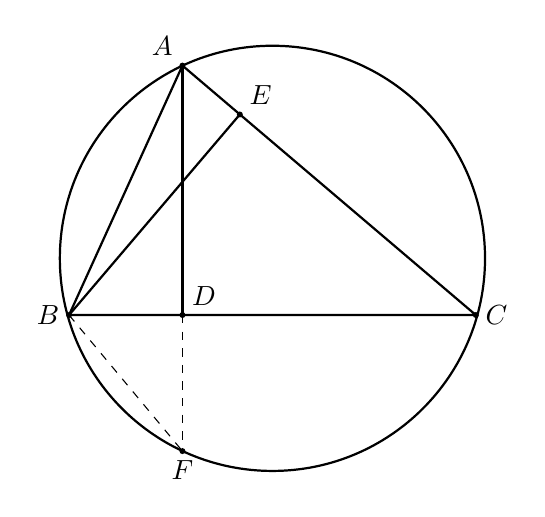
\begin{tikzpicture}[scale=0.9]
  \draw[thick] (0,0) circle (3);
  \coordinate (A) at (-1.27,2.72);
  \coordinate (B) at (-2.87,-0.8);
  \coordinate (C) at (2.87,-0.8);
  \coordinate (D) at (-1.27,-0.8);
  \coordinate (E) at (-0.46,2.03);
  \coordinate (F) at (-1.27,-2.72);
  \draw[thick] (A)--(B)--(C)--cycle;
  \draw[thick] (B)--(E);
  \draw[thick] (A)--(D);
  \draw[dashed] (D)--(F);
  \draw[dashed] (B)--(F);
  \fill (A) circle (1.2pt) node[above left] {$A$};
  \fill (B) circle (1.2pt) node[left] {$B$};
  \fill (C) circle (1.2pt) node[right] {$C$};
  \fill (D) circle (1.2pt) node[above right] {$D$};
  \fill (E) circle (1.2pt) node[above right] {$E$};
  \fill (F) circle (1.2pt) node[below] {$F$};
\end{tikzpicture}
\end{center}
\nopagebreak[4]
\Needspace{4\baselineskip}
\textbf{解析}
\nopagebreak[4]
\begin{center}% 1977 年广西百色卷（文科）第 3 题：圆内接三角形 ABC，AD、BE 分别为 BC、AC 边上的高，
% AD 延长交外接圆于 F，虚线 DF、BF（按源卷第 3 页布局：A 左上、B 左、C 右、F 底部，E 在 AC 上近 A，D 在 BC 上）
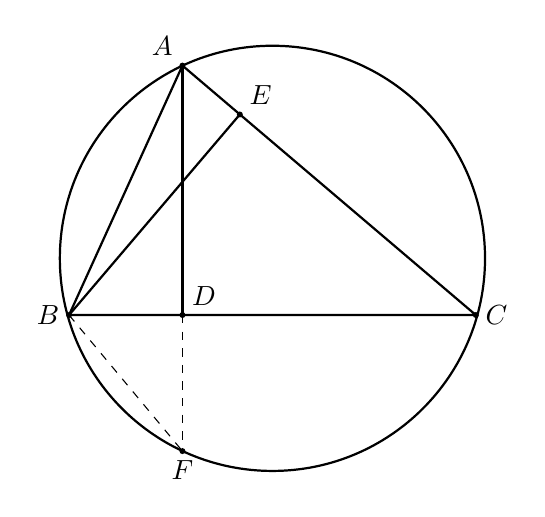
\begin{tikzpicture}[scale=0.9]
  \draw[thick] (0,0) circle (3);
  \coordinate (A) at (-1.27,2.72);
  \coordinate (B) at (-2.87,-0.8);
  \coordinate (C) at (2.87,-0.8);
  \coordinate (D) at (-1.27,-0.8);
  \coordinate (E) at (-0.46,2.03);
  \coordinate (F) at (-1.27,-2.72);
  \draw[thick] (A)--(B)--(C)--cycle;
  \draw[thick] (B)--(E);
  \draw[thick] (A)--(D);
  \draw[dashed] (D)--(F);
  \draw[dashed] (B)--(F);
  \fill (A) circle (1.2pt) node[above left] {$A$};
  \fill (B) circle (1.2pt) node[left] {$B$};
  \fill (C) circle (1.2pt) node[right] {$C$};
  \fill (D) circle (1.2pt) node[above right] {$D$};
  \fill (E) circle (1.2pt) node[above right] {$E$};
  \fill (F) circle (1.2pt) node[below] {$F$};
\end{tikzpicture}
\end{center}
\nopagebreak[4]
\Needspace{5\baselineskip}
\textbf{证法一}（与源卷证法一相同，独立复算一致）：在 $\triangle BEC$ 和 $\triangle ADC$ 中，因为 $BE\perp AC$、$AD\perp BC$，所以

\nopagebreak[4]
\[
\angle BEC=\angle ADC=90^\circ,
\]

\Needspace{5\baselineskip}
又 $\angle C$ 为公共角，故

\nopagebreak[4]
\[
\triangle BEC\sim\triangle ADC
\quad\Longrightarrow\quad
\angle EBC=\angle DAC.
\]

\Needspace{5\baselineskip}
因为 $F$ 在 $AD$ 的延长线上，所以 $\angle DAC=\angle FAC$；又 $A\text{、}B\text{、}C\text{、}F$ 四点共圆，$\angle FAC$ 与 $\angle FBC$ 是同弧 $FC$ 上的圆周角，故

\nopagebreak[4]
\[
\angle FAC=\angle FBC.
\]

\Needspace{5\baselineskip}
因此

\nopagebreak[4]
\[
\angle EBC=\angle FBC.
\]

\Needspace{5\baselineskip}
\textbf{证法二}（源卷另证，复算一致）：在 $\triangle BEC$ 和 $\triangle BFD$ 中，因为 $BE\perp AC$、$AD\perp BC$ 且 $F$ 在 $AD$ 的延长线上，所以

\nopagebreak[4]
\[
\angle BEC=\angle BDF=90^\circ;
\]

\Needspace{5\baselineskip}
又 $\angle C$ 与 $\angle F$ 是同弧 $AB$ 上的圆周角，

\nopagebreak[4]
\[
\angle C=\angle F.
\]

\Needspace{5\baselineskip}
于是 $\triangle BEC\sim\triangle BFD$，从而

\nopagebreak[4]
\[
\angle EBC=\angle FBD.
\]

因为 $D$ 在边 $BC$ 上，$\angle FBD=\angle FBC$，所以 $\angle EBC=\angle FBC$。

\gkanswer{答案：见解析版}

\end{answer}
\begin{answer}
\gksolhead{4}{}

\textbf{题目}：

红星农场一块地，用一台拖拉机来耕 $6$ 天，完成一半，后来加入了另一台新式拖拉机，两台合耕两天就耕完余下的地，新式拖拉机单独耕这块地要几天？

\Needspace{4\baselineskip}
\textbf{解析}

\Needspace{5\baselineskip}
旧拖拉机 $6$ 天耕完这块地的一半，故它每天耕这块地的 $\dfrac{1}{12}$。设新式拖拉机单独耕完这块地需 $x$ 天，则它每天耕 $\dfrac{1}{x}$。两台合耕 $2$ 天耕完余下的一半，依题意

\nopagebreak[4]
\[
2\left(\frac{1}{x}+\frac{1}{12}\right)=\frac{1}{2},
\]

\Needspace{5\baselineskip}
即

\nopagebreak[4]
\[
\frac{1}{x}+\frac{1}{12}=\frac{1}{4},
\qquad
\frac{1}{x}=\frac{1}{4}-\frac{1}{12}=\frac{1}{6},
\]

解得 $x=6$。故新式拖拉机单独耕完这块地需要 $6$ 天。

\begin{gktip}
\textbf{源注}：源卷另给「解法二」设每天耕地份额 $x$，方程为 $2\left(x+\frac{1}{12}\right)=\frac{1}{2}$，得 $x=\frac{1}{6}$，再由 $1\div\frac{1}{6}=6$（天）收尾；该式在源卷中把右括号错位印在等号之后，系排印错位，不影响题意。
\end{gktip}

\gkanswer{答案：$6$ 天。}

\end{answer}
\begin{answer}
\gksolhead{5}{}

\textbf{题目}：

曙光人民公社养鸡场，准备在鸡舍后面开辟一个矩形养鸡场，现仓库里有 $38$ 米长的铁丝网，问鸡场的长和宽各是多少米？才能使鸡场的面积最大？（靠鸡舍一边不围网）

\Needspace{4\baselineskip}
\textbf{解析}

\Needspace{5\baselineskip}
设垂直于鸡舍的一边（宽）为 $x$ 米，则平行于鸡舍的一边（长）为 $(38-2x)$ 米。设鸡场面积为 $S$ 平方米，则

\nopagebreak[4]
\[
S=x(38-2x)=-2x^2+38x.
\]

\Needspace{5\baselineskip}
二次项系数 $a=-2<0$，故 $S$ 有最大值，且在

\nopagebreak[4]
\[
x=-\frac{b}{2a}=-\frac{38}{2\times(-2)}=9.5
\]

\Needspace{5\baselineskip}
处取得。此时

\nopagebreak[4]
\[
38-2x=38-2\times9.5=19,
\]

\nopagebreak[4]
\[
S_{\max}=9.5\times19=180.5.
\]

故鸡场的宽为 $9.5$ 米、长为 $19$ 米时面积最大，最大面积为 $180.5$ 平方米。

\gkanswer{答案：长 $19$ 米、宽 $9.5$ 米，此时面积最大，为 $180.5\ \mathrm{m^2}$。}

\end{answer}
\begin{answer}
\gksolhead{6}{}

\textbf{题目}：

已知一个动点 $P(x,y)$ 到两定点 $A(1,3)$ 和 $B(-3,5)$ 的距离相等，求这动点的轨迹方程。

\Needspace{4\baselineskip}
\textbf{解析}

\Needspace{5\baselineskip}
由 $|PA|=|PB|$，即

\nopagebreak[4]
\[
\sqrt{(x-1)^2+(y-3)^2}=\sqrt{(x+3)^2+(y-5)^2}.
\]

\Needspace{5\baselineskip}
两边平方：

\nopagebreak[4]
\[
(x-1)^2+(y-3)^2=(x+3)^2+(y-5)^2.
\]

\Needspace{5\baselineskip}
展开：

\nopagebreak[4]
\[
x^2-2x+1+y^2-6y+9=x^2+6x+9+y^2-10y+25,
\]

\Needspace{5\baselineskip}
化简得

\nopagebreak[4]
\[
-2x-6y+10=6x-10y+34,
\]

\Needspace{5\baselineskip}
即

\nopagebreak[4]
\[
2x-y+6=0.
\]

故所求动点轨迹（线段 $AB$ 的垂直平分线）的方程为 $2x-y+6=0$。

\gkanswer{答案：$2x-y+6=0$。}

\end{answer}